\documentclass{beamer}

\usetheme{simple}

\usepackage{lmodern}
\usepackage[scale=2]{ccicons}

\usepackage{bussproofs}

\usepackage{mathpartir}

\usepackage{tikz}
\usetikzlibrary{arrows,positioning}
\tikzset{
    %Define standard arrow tip
    >=stealth',
    %Define style for boxes
    punkt/.style={
           rectangle,
           rounded corners,
           draw=black,
           text width=7.5em,
           minimum height=2em,
           text centered},
    % Define arrow style
    pil/.style={
           ->,
           thick,
           shorten <=2pt,
           shorten >=2pt,}
}



\title{On the Lambek Calculus with an Exchange Modality}
\subtitle{}
\date{July 7, 2018}
\author{Jiaming Jiang$^1$, Harley Eades III$^2$, Valeria de Paiva$^3$}
\institute{$^1$North Carolina State University; $^2$Augusta University; $^3$Nuance Communications}

\begin{document}

\maketitle



%--------------------------------------------------
% 1.a. Objective (a)
%--------------------------------------------------
\begin{frame}{Objective}

Linear logic uses the of-course modality, $!A$, to isolate
\textit{weakening} and \textit{contraction}:
$$\mbox{Weakening: }!A \rightarrow I$$
$$\mbox{Contraction: }!A \rightarrow !A \otimes !A$$

\invisible{
\begin{block}{Exchange Modality}
To isolate \textit{exchange} using a modality, $eA$:
\begin{gather*}
eA\otimes eB\multimap eB\otimes eA
\end{gather*}
\end{block}
}

\end{frame}


%--------------------------------------------------
% 1.b. Objective (b)
%--------------------------------------------------
\begin{frame}{Objective}

Linear logic uses the of-course modality, $!A$, to isolate
\textit{weakening} and \textit{contraction}:
$$\mbox{Weakening: }!A \rightarrow I$$
$$\mbox{Contraction: }!A \rightarrow !A \otimes !A$$

\begin{block}{Exchange Modality}
To isolate \textit{exchange} using a modality, $eA$:
\begin{gather*}
eA\otimes eB\multimap eB\otimes eA
\end{gather*}
\end{block}

\end{frame}


%--------------------------------------------------
% 2. Motivation
%--------------------------------------------------
\begin{frame}{Motivation}

In process calculi, to model sequential composition of processes:

\begin{columns}
\column{.4\textwidth}
  \begin{block}{$A\otimes B$}
  \begin{itemize}
  \item Commutative tensor product
  \item Processes $A$ and $B$ run in parallel
  \end{itemize}
  \end{block}
\column{.4\textwidth}
  \begin{block}{$A\triangleright B$}
  \begin{itemize}
  \item Non-commutative tensor product
  \item Process $A$ runs first, then process $B$
  \end{itemize}
  \end{block}
\end{columns}

\end{frame}

%--------------------------------------------------
% 3. Basic Approach
%--------------------------------------------------
\begin{frame}{Basic Approach}

Abstract Benton's Linear/Non-Linear (LNL) model:
\begin{itemize}
\item Remove the exchange structural rule: implicit in
      $\Phi,\Psi;\Gamma,\Delta$
\item Two logics:
      \begin{itemize}
      \item Intuitionistic linear logic
      \item Lambek Calculus
      \end{itemize}
\end{itemize}

\end{frame}


%--------------------------------------------------
% 4.a. LNL Model (a)
%--------------------------------------------------
\begin{frame}{Linear/Non-Linear Model}

A symmetric monoidal adjunction $F\dashv G$:
\begin{itemize}
\item Counit: $\varepsilon:FG\rightarrow id_\mathcal{C}$
\item Unit: $\eta:id_\mathcal{L}\rightarrow GF$
\end{itemize}

\begin{center}
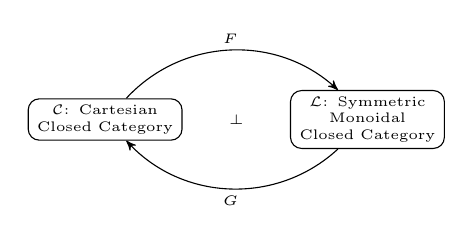
\begin{tikzpicture}[node distance=0.5cm, auto,]
  \tiny
  \node (adjoint) {$\perp$};
  \node[punkt,left=of adjoint] (ccc) {$\mathcal{C}$: Cartesian Closed Category};
  \node[punkt,right=of adjoint] (smcc) {$\mathcal{L}$: Symmetric Monoidal Closed Category}
    edge[<-,bend right=45] node[above] {$F$} (ccc)
    edge[->,bend left=45] node[auto] {$G$} (ccc);
\end{tikzpicture}
\end{center}

\invisible{
\begin{block}{}
\begin{itemize}
\item Monad $(GF,\eta,\mu=G\varepsilon_F)$ on the CCC: strong and
      commutative
\item Comonad $(FG,\varepsilon,\delta=F\eta_G)$ on the SMCC: symmetric
      monoidal
\item Of-course modality: $!=FG$
\end{itemize}
\end{block}
}

\end{frame}


%--------------------------------------------------
% 4.b. LNL Model (b)
%--------------------------------------------------
\begin{frame}{Linear/Non-Linear Model}

A symmetric monoidal adjunction $F\dashv G$:
\begin{itemize}
\item Counit: $\varepsilon:FG\rightarrow id_\mathcal{C}$
\item Unit: $\eta:id_\mathcal{L}\rightarrow GF$
\end{itemize}

\begin{center}
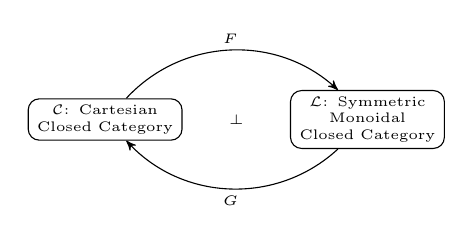
\begin{tikzpicture}[node distance=0.5cm, auto,]
  \tiny
  \node (adjoint) {$\perp$};
  \node[punkt,left=of adjoint] (ccc) {$\mathcal{C}$: Cartesian Closed Category};
  \node[punkt,right=of adjoint] (smcc) {$\mathcal{L}$: Symmetric Monoidal Closed Category}
    edge[<-,bend right=45] node[above] {$F$} (ccc)
    edge[->,bend left=45] node[auto] {$G$} (ccc);
\end{tikzpicture}
\end{center}

\begin{block}{}
\begin{itemize}
\item Monad $(GF,\eta,\mu=G\varepsilon_F)$ on the CCC: strong and
      commutative
\item Comonad $(FG,\varepsilon,\delta=F\eta_G)$ on the SMCC: symmetric
      monoidal
\item Of-course modality: $!=FG$
\end{itemize}
\end{block}

\end{frame}


%--------------------------------------------------
% 5.a. CNC Model (a)
%--------------------------------------------------
\begin{frame}{Commutative/Non-Commutative (CNC) Model}

\begin{center}
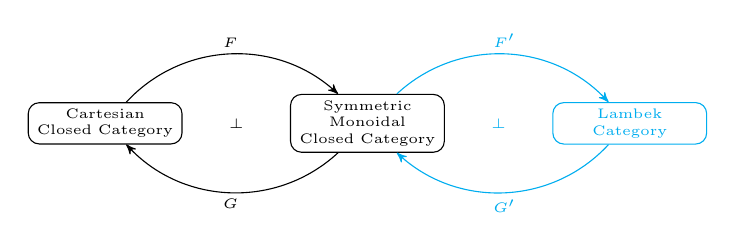
\begin{tikzpicture}[node distance=0.5cm, auto,]
  \tiny
  \node (adjoint1) {$\perp$};
  \node[punkt,left=of adjoint1] (ccc) {Cartesian Closed Category};
  \node[punkt,right=of adjoint1] (smcc) {Symmetric Monoidal Closed Category}
    edge[<-,bend right=45] node[above] {$F$} (ccc)
    edge[->,bend left=45] node[auto] {$G$} (ccc);
  \node[right=of smcc,cyan] (adjoint2) {$\perp$};
  \node[punkt,right=of adjoint2,cyan] (lambek) {Lambek Category}
    edge[<-,bend right=45,cyan] node[above] {$F'$} (smcc)
    edge[->,bend left=45,cyan] node[auto] {$G'$} (smcc);
\end{tikzpicture}
\end{center}

\end{frame}


%--------------------------------------------------
% 5.b. CNC Model (b)
%--------------------------------------------------
\begin{frame}{Commutative/Non-Commutative (CNC) Model}

A monoidal adjunction $F\dashv G$:
\begin{itemize}
\item Counit: $\varepsilon:FG\rightarrow id_\mathcal{C}$
\item Unit: $\eta:id_\mathcal{L}\rightarrow GF$
\end{itemize}

\begin{center}
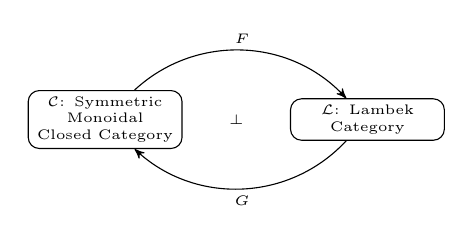
\begin{tikzpicture}[node distance=0.5cm, auto,]
  \tiny
  \node (adjoint) {$\perp$};
  \node[punkt,left=of adjoint] (smcc) {$\mathcal{C}$: Symmetric Monoidal Closed Category};
  \node[punkt,right=of adjoint] (lambek) {$\mathcal{L}$: Lambek Category}
    edge[<-,bend right=45] node[above] {$F$} (smcc)
    edge[->,bend left=45] node[auto] {$G$} (smcc);
\end{tikzpicture}
\end{center}

\invisible{
\begin{block}{}
\begin{itemize}
\item Monad $(GF,\eta,\mu=G\varepsilon_F)$ on the SMCC: strong but
      non-commutative
\item Comonad $(FG,\varepsilon,\delta=F\eta_G)$ on the Lambek category:
      monoidal
\item Exchange: a natural transformation
      $\mathrm{ex}^{FG}:A\triangleright B\rightarrow B\triangleright A$ in
      the co-Eilenberg-Moore category $\mathcal{L}^{FG}$ of the comonad \\
      $\Rightarrow$: $\mathcal{L}^{FG}$ is symmetric monoidal 
\end{itemize}
\end{block}
}

\end{frame}


%--------------------------------------------------
% 5.c. CNC Model (c)
%--------------------------------------------------
\begin{frame}{Commutative/Non-Commutative (CNC) Model}

A monoidal adjunction $F\dashv G$:
\begin{itemize}
\item Counit: $\varepsilon:FG\rightarrow id_\mathcal{C}$
\item Unit: $\eta:id_\mathcal{L}\rightarrow GF$
\end{itemize}

\begin{center}
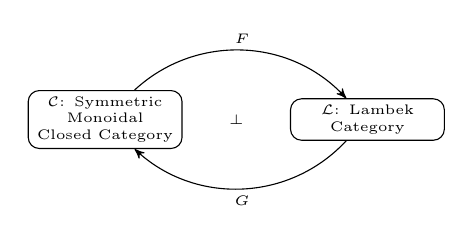
\begin{tikzpicture}[node distance=0.5cm, auto,]
  \tiny
  \node (adjoint) {$\perp$};
  \node[punkt,left=of adjoint] (smcc) {$\mathcal{C}$: Symmetric Monoidal Closed Category};
  \node[punkt,right=of adjoint] (lambek) {$\mathcal{L}$: Lambek Category}
    edge[<-,bend right=45] node[above] {$F$} (smcc)
    edge[->,bend left=45] node[auto] {$G$} (smcc);
\end{tikzpicture}
\end{center}

\begin{block}{}
\begin{itemize}
\item Monad $(GF,\eta,\mu=G\varepsilon_F)$ on the SMCC: strong but
      non-commutative
\item Comonad $(FG,\varepsilon,\delta=F\eta_G)$ on the Lambek category:
      monoidal
\item Exchange: a natural transformation
      $\mathrm{ex}^{FG}:A\triangleright B\rightarrow B\triangleright A$ in
      the co-Eilenberg-Moore category $\mathcal{L}^{FG}$ of the comonad \\
      $\Rightarrow$: $\mathcal{L}^{FG}$ is symmetric monoidal 
\end{itemize}
\end{block}

\end{frame}


%--------------------------------------------------
% 6. CNC Logic
%--------------------------------------------------
\begin{frame}{CNC Logic}

\begin{itemize}
\item Left: intuitionistic linear logic
\item Right: mixed commutative/non-commutative Lambek calculus
\end{itemize}

\begin{center}
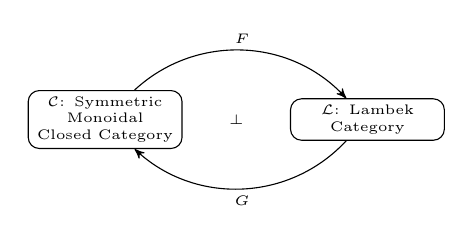
\begin{tikzpicture}[node distance=0.5cm, auto,]
  \tiny
  \node (adjoint) {$\perp$};
  \node[punkt,left=of adjoint] (smcc) {$\mathcal{C}$: Symmetric Monoidal Closed Category};
  \node[punkt,right=of adjoint] (lambek) {$\mathcal{L}$: Lambek Category}
    edge[<-,bend right=45] node[above] {$F$} (smcc)
    edge[->,bend left=45] node[auto] {$G$} (smcc);
  \scriptsize
\end{tikzpicture}
\end{center}

\end{frame}

%--------------------------------------------------
% 7. CNC Logic: Notation
%--------------------------------------------------
\begin{frame}{CNC Logic: Notation}

\begin{columns}
\column{0.47\textwidth}
  \centerline{\textbf{Intuitionistic Linear Logic}}

  $\mathcal{C}$-Types: $W$, $X$, $Y$, $Z$ \\
  $\mathcal{C}$-Terms: $t$ \\
  $\mathcal{C}$-Contexts: $\Phi$, $\Psi$ \\
  $\mathcal{C}$-Typing Judgment: $\Phi,\Psi \vdash_\mathcal{C} t:X$

\column{0.47\textwidth}
  \centerline{\textbf{Lambek Calculus}}

  $\mathcal{L}$-Types: $A$, $B$, $C$, $D$ \\
  $\mathcal{L}$-Terms: $s$ \\
  $\mathcal{L}$-Contexts: $\Gamma$, $\Delta$ \\
  $\mathcal{L}$-Typing Judgment: $\Gamma;\Delta \vdash_\mathcal{L} s:A$
\end{columns}

\end{frame}


%--------------------------------------------------
% 8.a. CNC Logic: Example Typing Rules (a)
%--------------------------------------------------
\begin{frame}{CNC Logic: Example Typing Rules}

Exchange rules:
\begin{prooftree}
\scriptsize
\AxiomC{$\Phi,x:X,y:Y,\Psi \vdash_\mathcal{C} t:Z$}
\LeftLabel{}\RightLabel{$\mathcal{C}$-$\mathsf{ex}$}
\UnaryInfC{$\Phi,z:Y,w:X,\Psi \vdash_\mathcal{C} \mathsf{ex}\ w,z\ \mathsf{with}\ x,y\ \mathsf{in}\ t:Z$}
\end{prooftree}

\begin{prooftree}
\scriptsize
\AxiomC{$\Gamma;x:X;y:Y;\Delta \vdash_\mathcal{L} s:A$}
\LeftLabel{}\RightLabel{$\mathcal{L}$-$\mathsf{ex}$}
\UnaryInfC{$\Gamma;z:Y;w:X;\Delta \vdash_\mathcal{L} \mathsf{ex}\ w,z\ \mathsf{with}\ x,y\ \mathsf{in}\ s:A$}
\end{prooftree}

%Cut rules:
%  \begin{prooftree}
%  \scriptsize
%  \AxiomC{$\Phi\vdash_\mathcal{C}t_1:X$}
%  \AxiomC{$\Psi_1,x:X,\Psi_2\vdash_\mathcal{C}t2:Y$}
%  \LeftLabel{}\RightLabel{$\mathcal{C}$-$\mathrm{Cut}$}
%  \BinaryInfC{$\Psi_1,\Phi,\Psi_2\vdash_\mathcal{C}[t1/x]t2:Y$}
%  \end{prooftree}
%
%  \begin{prooftree}
%  \scriptsize
%  \AxiomC{$\Gamma\vdash_\mathcal{L}s_1:A$}
%  \AxiomC{$\Delta_1;x:X;\Delta_2\vdash_\mathcal{L}s2:B$}
%  \LeftLabel{}\RightLabel{$\mathcal{L}$-$\mathrm{Cut}$}
%  \BinaryInfC{$\Delta_1;\Gamma;\Delta_2\vdash_\mathcal{C}[s1/x]s2:B$}
%  \end{prooftree}
%
%  \begin{prooftree}
%  \scriptsize
%  \AxiomC{$\Phi\vdash_\mathcal{C}s:X$}
%  \AxiomC{$\Gamma_1;x:X;\Gamma_2\vdash_\mathcal{L}s:A$}
%  \LeftLabel{}\RightLabel{$\mathcal{LC}$-$\mathrm{Cut}$}
%  \BinaryInfC{$\Gamma_1;\Phi;\Gamma_2\vdash_\mathcal{C}[t/x]s:A$}
%  \end{prooftree}

\end{frame}


%--------------------------------------------------
% 8.b. CNC Logic: Example Typing Rules (b)
%--------------------------------------------------
\begin{frame}{CNC Logic: Example Typing Rules}


Functor rules for $\mathsf{G}$:
\begin{prooftree}
\scriptsize
\AxiomC{$\Phi\vdash_\mathcal{L}s:A$}
\LeftLabel{}\RightLabel{$\mathcal{C}$-$\mathsf{G}_I$}
\UnaryInfC{$\Phi\vdash_\mathcal{C}\mathsf{G}s:\mathsf{G}A$}
\end{prooftree}

\begin{prooftree}
\scriptsize
\AxiomC{$\Phi\vdash_\mathcal{C}t:\mathsf{G}A$}
\LeftLabel{}\RightLabel{$\mathcal{C}$-$\mathsf{G}_E$}
\UnaryInfC{$\Phi\vdash_\mathcal{L}\mathsf{derelict}\ t:A$}
\end{prooftree}

\invisible{
Functor rules for $\mathsf{F}$:
\begin{prooftree}
\scriptsize
\AxiomC{$\Phi\vdash_\mathcal{C}t:X$}
\LeftLabel{}\RightLabel{$\mathcal{L}$-$\mathsf{F}_I$}
\UnaryInfC{$\Phi\vdash_\mathcal{L}\mathsf{F}t:\mathsf{F}X$}
\end{prooftree}

\begin{prooftree}
\scriptsize
\AxiomC{$\Gamma\vdash_\mathcal{L}s_1:\mathsf{F}X$}
\AxiomC{$\Delta_1;x:X;\Delta_2\vdash_\mathcal{L}s_2:A$}
\LeftLabel{}\RightLabel{$\mathcal{L}$-$\mathsf{F}_E$}
\BinaryInfC{$\Delta_1;\Gamma;\Delta_2\vdash_\mathcal{L}\mathsf{let}\ s_1:\mathsf{F}X\ \mathsf{be}\ \mathsf{F}x\ \mathsf{in}\ s_2:A$}
\end{prooftree}
}

\end{frame}


%--------------------------------------------------
% 8.c. CNC Logic: Example Typing Rules (c)
%--------------------------------------------------
\begin{frame}{CNC Logic: Example Typing Rules}


Functor rules for $\mathsf{G}$:
\begin{prooftree}
\scriptsize
\AxiomC{$\Phi\vdash_\mathcal{L}s:A$}
\LeftLabel{}\RightLabel{$\mathcal{C}$-$\mathsf{G}_I$}
\UnaryInfC{$\Phi\vdash_\mathcal{C}\mathsf{G}s:\mathsf{G}A$}
\end{prooftree}

\begin{prooftree}
\scriptsize
\AxiomC{$\Phi\vdash_\mathcal{C}t:\mathsf{G}A$}
\LeftLabel{}\RightLabel{$\mathcal{C}$-$\mathsf{G}_E$}
\UnaryInfC{$\Phi\vdash_\mathcal{L}\mathsf{derelict}\ t:A$}
\end{prooftree}

Functor rules for $\mathsf{F}$:
\begin{prooftree}
\scriptsize
\AxiomC{$\Phi\vdash_\mathcal{C}t:X$}
\LeftLabel{}\RightLabel{$\mathcal{L}$-$\mathsf{F}_I$}
\UnaryInfC{$\Phi\vdash_\mathcal{L}\mathsf{F}t:\mathsf{F}X$}
\end{prooftree}

\begin{prooftree}
\scriptsize
\AxiomC{$\Gamma\vdash_\mathcal{L}s_1:\mathsf{F}X$}
\AxiomC{$\Delta_1;x:X;\Delta_2\vdash_\mathcal{L}s_2:A$}
\LeftLabel{}\RightLabel{$\mathcal{L}$-$\mathsf{F}_E$}
\BinaryInfC{$\Delta_1;\Gamma;\Delta_2\vdash_\mathcal{L}\mathsf{let}\ s_1:\mathsf{F}X\ \mathsf{be}\ \mathsf{F}x\ \mathsf{in}\ s_2:A$}
\end{prooftree}

\end{frame}


%--------------------------------------------------
% 9. CNC Logic: Other Results
%--------------------------------------------------
\begin{frame}{CNC Logic: Other Results}

\begin{itemize}
\item $\beta$-reductions: one step $\beta$-reduction rules
\item Commuting conversions
\item Cut elimination
\item Equivalence between sequent calculus and natural deduction
\item Strong normalization via a translation to LNL logic
\item A concrete model in dialectica categories
\end{itemize}

\end{frame}


%--------------------------------------------------
% 10. Conclusion
%--------------------------------------------------
\begin{frame}{Conclusion}

\begin{itemize}
\item Commutative/Non-commutative Logic:
      \begin{itemize}
      \item Left: intuitionistic linear logic
      \item Right: Lambek calculus
      \end{itemize}
\item Categorical model: a monoidal adjunction
      \begin{itemize}
      \item Left: symmetric monoidal closed category
      \item Right: Lambek category
      \end{itemize}
\end{itemize}

\begin{block}{Exchange Natural Transformation}
$\mathrm{ex}^{FG}:A\triangleright B\rightarrow B\triangleright A$ in the
co-Eilenberg-Moore category $\mathcal{L}^{FG}$ of the comonad on the Lambek
category
\end{block}

\end{frame}


\end{document}


















